\section{Preliminary Evaluation}\label{sec:prelim}
% provenance: jrn_01KXTX3PH43VR78AM1GZHC27T1 (real in-session results: credsvc + OpenDSS).
% All numbers here are measured, at reduced scale; the full pre-registered sweep remains future work.

We report a preliminary evaluation that exercises the full pipeline end to end and produces
measured results. Its scope is deliberately limited and stated plainly: a workstation platform
(no constrained hardware), the real IEEE~8500-node feeder as a first benchmark run but not yet the
PNNL 9500 system, a single solver (OpenDSS, no GridLAB-D cross-check), load-state snapshots rather
than a full seasonal time series, one PV penetration level, a fixed rather than per-state-optimized
attacker, and a Python IEEE~2030.5-style client in place of the EPRI C client. These results
establish that the mechanism and the measurement work; the pre-registered full-scale sweep is not
replaced by them. Table~\ref{tab:implstatus} states the status of each component.

\begin{table}[t]
\centering
\caption{Implementation and evaluation status.}
\label{tab:implstatus}
\small
\begin{tabular}{@{}p{0.62\columnwidth}p{0.28\columnwidth}@{}}
\toprule
Component & Status \\
\midrule
Cyber-side analysis engine & implemented, measured \\
Credential service (issuance, fresh key, session/command enforcement) & implemented, measured \\
Feeder co-simulation (OpenDSS, two feeders) & implemented, measured \\
Availability fault injection & implemented, measured \\
Native EPRI-client 2030.5 traffic & planned \\
Constrained-hardware / TEE attestation & planned \\
GridLAB-D cross-solver check & planned \\
Interoperability tests & planned \\
Full pre-registered sweep & planned \\
\bottomrule
\end{tabular}
\end{table}

\paragraph{Functional invariants and containment (C1, C2).}
The credential service uses real X.509 / ECDSA certificates and an EAT-style attestation token.
Ten implemented security invariants all pass: bootstrap identity cannot authorize control,
issuance requires a valid fresh attestation, the certificate is bound to a freshly generated
operational key, replayed evidence is rejected, an expired credential cannot issue commands,
per-command scope matches issuance, a bad measurement yields only a narrowed safe-mode scope, a
prior epoch cannot self-renew, and a copied prior operational key is contained at the next epoch.
With per-command revalidation the post-expiry acceptance gap is
$\Delta_{\mathrm{expiry}} = -0.5$\,s (the last accepted adversarial command precedes expiry),
against $+5.0$\,s without enforcement, where it grows to the cached session age. A fresh
operational key is generated each epoch, so a copied key is useless after rotation.
Table~\ref{tab:invariants} lists the invariants and their outcomes.

\begin{table}[t]
\centering
\caption{Security invariants (all pass on the prototype, real X.509/mTLS).}
\label{tab:invariants}
\small
\begin{tabular}{@{}p{0.06\columnwidth}p{0.74\columnwidth}c@{}}
\toprule
ID & Invariant & Result \\
\midrule
I1 & Bootstrap identity cannot authorize control & pass \\
I2 & Issuance requires a fresh attestation & pass \\
I3 & Credential bound to a fresh public key & pass \\
I4 & Replayed evidence rejected & pass \\
I5 & Expired credential cannot issue a command & pass \\
I6 & Scope enforced per command & pass \\
I7 & Bad measurement yields degraded/denied scope & pass \\
I8 & Prior epoch cannot self-renew & pass \\
I9 & Copied prior key fails after rotation & pass \\
I10 & Active session/command bounded past expiry & pass \\
\bottomrule
\end{tabular}
\end{table}

\paragraph{Overhead (C3).}
On the workstation tier, over 500 iterations (100 for the handshake), the median software-path
latencies (no hardware root of trust, no network transport) are
$0.015$\,ms for key generation, $0.05$\,ms for attestation construction, $0.2$\,ms for a full
attested issuance, and $1.1$\,ms for a real mutual-TLS handshake, with p99 tails within a few
milliseconds; the issuer sustains about $4900$ issuances per second single-threaded. Renewal is
therefore inexpensive on this platform. The measured operations are standard EC~P-256 primitives
dominated by a single ECDSA signature and verification, so per-issuance cost on a constrained
inverter controller can be estimated from its public-key throughput; a hardware-backed measurement
is declared future work rather than claimed here.

\paragraph{Availability (C6).}
Renewal is a full attested issuance, so its cost is the issuance cost above; the renewal safety
margin $T_{\mathrm{TTL}} - (T_{\mathrm{renew,p99}} + T_{\mathrm{net}})$ stays positive at every
tested lifetime down to five minutes, and a $100{,}000$-device fleet re-mints in about $20$\,s
single-threaded, so short lifetimes are latency-feasible. The availability risk is instead a
verifier or issuer outage longer than the credential lifetime. Injecting verifier outages into the
running service (renewal fails during the outage), fail-closed denial retains $0.77$ of legitimate
control availability over the outage window, a bounded grace period $0.83$, and degraded-scope safe
mode $1.0$; control recovers as soon as the verifier returns. The injection is in-process; a
networked or hardware outage, clock skew, and renewal storms remain for the full study.

\paragraph{Feeder consequence (C5).}
We run an export/overvoltage attack on the real IEEE~8500-node feeder (4876 buses, 1177 loads,
12\,MW) with 600 seeded rooftop-PV units, ten paired seeds, under three load states.
Table~\ref{tab:prelim} reports the attack-induced overvoltage-violation area $\Delta J_V$, the
median over seeds against the base case at the same load. Because the 8500 base has native
undervoltage at its extremities, we report the induced \emph{overvoltage} area the attack targets
rather than a two-sided area that would credit the attack for lifting sagging nodes; this
attack-specific endpoint was chosen after observing the base undervoltage, while the two-sided area
remains the declared primary system-level endpoint. Under light
load and high PV a legacy full-authorization compromise induces a median $\Delta J_V = 126.6$
(range $108$--$134$); the CONTAINDER narrowed scope keeps it within the ANSI band (median $\Delta J_V \le 0$). Under
normal load the figures are $6.6$ against $0.1$. Under heavy load the export attack cannot raise
voltage above the band, so $\Delta J_V \approx 0$ regardless of policy. The ephemeral-only baseline
equals the legacy one physically, since a short lifetime does not narrow scope; its advantage is
temporal. The consequence is strongly state dependent, the physical-state separation of
Proposition~3 on the real benchmark.

\paragraph{Time-series containment and mechanism decomposition (C5).}
% provenance: jrn_01KY13EQJ6V8AZCRHB944ZAZJY (real 8500 time-series).
To measure temporal containment directly, rather than as a product of a measured and a modeled
factor, we run each policy as one time-series: a compromised credential drives the DER from minute
five, and its lifecycle then determines whether the malicious setpoint keeps affecting the feeder.
We integrate the real induced overvoltage area over time, in p.u.-node-minutes
(Fig.~\ref{fig:timeseries}). A legacy credential (B1) holds the feeder in violation for the whole
horizon (integral $6956$, no recovery). Holding the broad scope fixed but adding the CONTAINDER
lifecycle (A4) halves the integral to $3196$ and the feeder recovers at credential expiry, which
isolates the temporal effect of lifetime with session and command enforcement at equal scope.
Removing session enforcement (A2) or command cleanup (A3) from that configuration returns the
feeder to no recovery ($7030$), so each mechanism is necessary. Narrowing scope (B5) additionally
bounds the instantaneous envelope, and the integral falls to $3.8$. This single experiment gives
the equal-scope decomposition the design intends: scope bounds the envelope, lifetime with
enforcement bounds the duration, and neither alone suffices.

\begin{figure}[t]
\centering
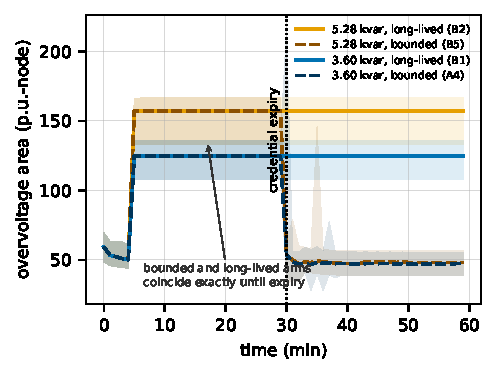
\includegraphics[width=\columnwidth]{figures/fig_timeseries.pdf}
\caption{Time-series induced overvoltage on the IEEE 8500-node feeder (light load, one seed).
A legacy credential (B1) never recovers; at the same broad scope the CONTAINDER lifecycle (A4)
recovers at credential expiry; narrow scope (B5) additionally bounds the instantaneous envelope.
The session-off and command-cleanup-off ablations track B1 and are omitted for clarity.}
\label{fig:timeseries}
\end{figure}

\paragraph{Policy comparison and the persistence--scope interaction (C5, H1).}
% provenance: jrn_01KXWJ4TPTK2DGSBKY5YCF50T5 (real 8500 full baseline + ablation sweep).
As a first-order summary that separates all six baselines at once, we also report a proxy
combining the measured physical envelope with the modeled retained authority,
$\Delta J_V \times \BRauth$ (Table~\ref{tab:exposure}); this is a physical-impact-times-duration
quantity, not the flexibility-time $\BRexp$ integral of the model, and the time-series above is the
direct measurement it approximates. At full authorization scope, lengthening persistence from the
ephemeral B3 (retained authority $\approx 10$\,h) to the legacy B1 ($\approx 2$\,years) multiplies
light-load exposure roughly $1700\times$, from $1.3\times10^3$ to $2.2\times10^6$. At narrow scope
the same change is inert: B2 and B5 are both near zero. The effect of persistence therefore
depends on scope, consistent with the pre-registered persistence-by-scope hypothesis; because
exposure is a product of a measured and a modeled factor, this preliminary pattern does not by
itself establish the pre-registered mixed-effects test over the full sweep. The full design B5 has lower exposure than both the ephemeral-only B3 and
the attestation-only B4 ($8.3\times10^3$), so neither half alone suffices. Mechanism ablations
attribute the reduction: removing scope narrowing restores physical exposure (from near zero to
$1.5\times10^3$), while fail-open renewal inflates retained authority from $12$\,h to
$1.75\times10^4$\,h. Scope narrowing bounds the physical envelope; attestation-gated renewal with
session and command enforcement bounds how long it persists, the temporal containment the C2
copied-key and session-theft results measure.

\begin{table}[t]
\centering
\caption{First-order exposure proxy $\Delta J_V\times\BRauth$ by baseline (light load, IEEE 8500, N{=}10; $\Delta J_V$ measured, $\BRauth$ modeled). The time-series (Fig.~\ref{fig:timeseries}) is the direct measurement.}
\label{tab:exposure}
\small
\begin{tabular}{@{}llcc@{}}
\toprule
Baseline & Scope & $\BRauth$ & Exposure \\
\midrule
B1 legacy full & full & $\sim$2\,yr & $2.2\times10^6$ \\
B2 ACL-narrow & narrow & $\sim$2\,yr & $\approx 0$ \\
B3 ephemeral-only & full & $\sim$10\,h & $1.3\times10^3$ \\
B4 attestation-only & reference & $\sim$14\,d & $8.3\times10^3$ \\
B5 full CONTAINDER & narrow & $\sim$12\,h & $\approx 0$ \\
B6 safe-mode & narrow & $\sim$12\,h & $\approx 0$ \\
\bottomrule
\end{tabular}
\end{table}

\begin{table}[t]
\centering
\caption{Attack-induced overvoltage-violation area $\Delta J_V$ on the IEEE 8500-node feeder (median over 10 seeds).}
\label{tab:prelim}
\small
\begin{tabular}{@{}lcc@{}}
\toprule
Operating state & Legacy full (B1) & CONTAINDER (B5) \\
\midrule
light load / high PV & 126.6 & $-0.01$ \\
normal & 6.6 & 0.13 \\
heavy load & $\approx 0$ & $\approx 0$ \\
\bottomrule
\end{tabular}
\end{table}

\begin{figure}[t]
\centering
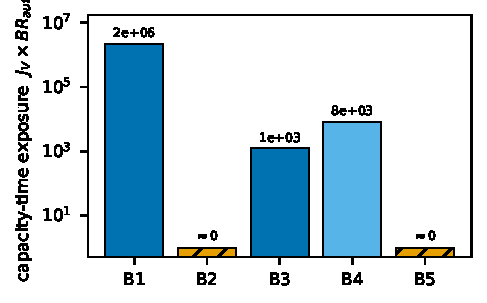
\includegraphics[width=\columnwidth]{figures/fig_exposure.pdf}
\caption{Capacity-time exposure by baseline on the IEEE 8500-node feeder (light load, log scale).
Persistence multiplies exposure only at full scope (B1 vs B3); at narrow scope (B2, B5) it is
inert, the persistence--scope interaction. Bars floored at 1 for log display; B2, B5, B6 are $\approx 0$.}
\label{fig:exposure}
\end{figure}

\begin{figure}[t]
\centering
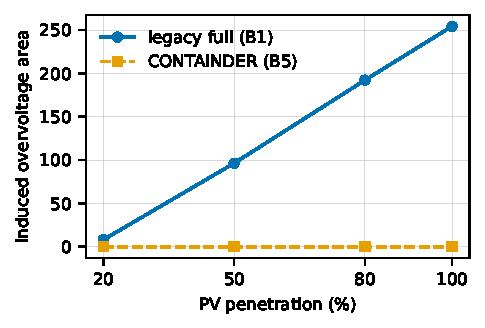
\includegraphics[width=\columnwidth]{figures/fig_penetration.pdf}
\caption{Induced overvoltage area versus PV penetration (IEEE 8500, light load, 5 seeds). Harm
scales with penetration under the legacy baseline; containment is penetration-independent under
CONTAINDER.}
\label{fig:penetration}
\end{figure}

\begin{figure}[t]
\centering
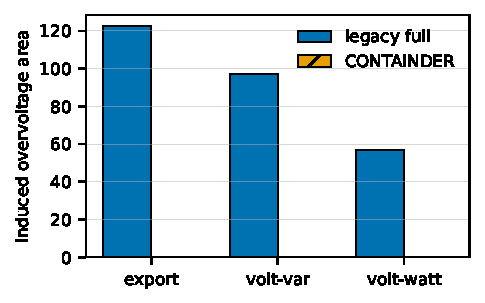
\includegraphics[width=\columnwidth]{figures/fig_attack_families.pdf}
\caption{Induced overvoltage area by attack family (IEEE 8500, light load). Narrowing scope
contains overvoltage driven by active or reactive authority.}
\label{fig:families}
\end{figure}

\paragraph{Penetration and robustness.}
Induced overvoltage grows with PV penetration under a legacy full-authorization compromise, from
$8$ at $20\%$ to $254$ at $100\%$, while the CONTAINDER narrowed scope holds it near zero at every
level (Fig.~\ref{fig:penetration}). The same containment holds across attack families
(Fig.~\ref{fig:families}), and capacity-time exposure separates all six baselines along the
persistence--scope interaction (Fig.~\ref{fig:exposure}). It also holds on a second public feeder:
on the IEEE~123-bus system a legacy full-authorization compromise induces overvoltage under high PV
penetration (induced area up to $2.2$) that CONTAINDER holds at zero, though the stiffer regulated
$4.16$\,kV feeder requires higher penetration than the 8500 to breach the band, consistent with the
feeder-dependence of Proposition~3.

\paragraph{Attack families.}
% provenance: jrn_01KXWJDXAC3N56E0477DDH5MMD (real 8500 attack-family sweep).
The containment holds across attack families, not only the export attack (five seeds, light
load). A legacy full-authorization compromise induces overvoltage areas of $122$ (export-limit),
$97$ (volt-var, reactive injection alone), and $57$ (volt-watt, active injection) that the
CONTAINDER narrowed scope reduces to zero in every case; for a curtailment-spam attack, narrowing
cuts the per-node voltage variability from $0.012$ to $0.004$\,p.u., a factor of three.
Overvoltage is reachable through active or reactive authority, and narrowing scope removes both.

\paragraph{Least privilege preserves legitimate utility (C5).}
A scope that removed all control would contain the attack trivially, by disabling the device.
CONTAINDER's operational scope is bounded volt-var support, not read-only. Under it a legitimate
reactive voltage-support command is authorized while an active-power export command is denied; the
attacker's only remaining lever is bounded reactive, which induces overvoltage $0.04$ against $126$
under full authorization, whereas a read-only scope authorizes neither the legitimate nor the
malicious command. The narrow scope therefore retains the most common legitimate DER function while
bounding the attack, which distinguishes least privilege from denial of service.

\paragraph{Limitations.}
These results are preliminary and we do not generalize them. Physical results come from two public feeders
(a ten-seed IEEE 8500 sweep and a confirmatory IEEE 123 run) and a single solver, with a fixed
export attacker; the IEEE 9500-node system was obtained
but did not converge in our OpenDSS build and is deferred to an appendix tier per the study's
pre-registered contingency. Retained-authority figures are model outputs under assumed attestation
and lifetime parameters, not measured field values, and the exposure metric inherits those
assumptions. The availability results model the outage response rather than injecting real verifier
outages on hardware. Incremental deployment is by construction; interoperability against an
unmodified endpoint is untested. The pre-registered sweep on two public feeders, with a
cross-solver check, seasonal states, constrained hardware, and the full seed budget, is what would
support quantitative claims; the 8500-node results are the primary feeder evidence here.
